\documentclass[a4paper,10pt]{article}
\usepackage[utf8]{inputenc}
\usepackage[T1]{fontenc}
\usepackage[english]{babel}
\usepackage[a4paper,top=2.5cm, bottom=2.5cm, left=2.5cm, right=2.5cm]{geometry}
\usepackage{graphicx}
\usepackage{lscape}

\title{Software Architectures\\ Assignment 3 : Service Oriented Architectures - Web Services}
\author{Arnaud Rosette, Simon Picard}

\begin{document}
\maketitle
\section{Exercise 1 : BPEL Processes}
\subsection{BPEL}
-The order of operations must be modified in order to parallelize the invocation of the web services. The two "AssignSearchRequest" have to be executed one  after the other to be able to perform the invocations in parallel. Once this is done, BPEL provides a flow construction which allows tasks to be executed simultaneously. There was a small error in the "AssigneSearchRequest", to copy the query, the original process used "string(\$request.body\/\/query)" but the correct form is "string(\$request.body\/\/tns:query)".\\

-There are two sections of the main process which are executed in parallel, one where the response page and the search requests are set up and another where the calls to the library are actually done. It is clear that these calls could not be performed earlier because they need their parameter to be set which is done in the preparation of the search requests. Therefore, the "AssignSearchRequest" share data dependencies with the invocations of the web services. And, of course, the next part of the process, where the results of the library searches are written in the response and then the response is sent, is sequential.\\

-In the flow structure, links can be used to state some control dependencies, in our case we could link the parts where parameter for a call are set to the call itself, stating that tasks can be executed simultaneously but these two operations have to be performed in a certain order.
\subsection{Querying web services}
-Here is an example of a result of the service.
\begin{verbatim}
<searchBooksResponse xmlns="urn:soft.vub.ac.be/" xmlns:xsd="http://www.w3.org/2001/XMLSchema"
        xmlns:xsi="http://www.w3.org/2001/XMLSchema-instance">
    <book xmlns="">
        <author>Jordan Belfort</author>
        <year>2008</year>
        <isbn>606259090</isbn>
        <language>en</language>
        <publisher>Hodder Paperback</publisher>
        <title>The Wolf of Wall Street</title>
    </book>
</searchBooksResponse>
<searchForBooksReturn xmlns="http://library.be" xmlns:xsd="http://www.w3.org/2001/XMLSchema" 
        xmlns:xsi="http://www.w3.org/2001/XMLSchema-instance">
    <author>James, E. L.</author>
    <date>3914-01-10T23:00:00.000Z</date>
    <isbn>0345803485</isbn>
    <language>English</language>
    <publisher>Vintage Books</publisher>
    <title>50 Shades of Grey</title>
</searchForBooksReturn>
\end{verbatim}
The responses share attributes such as author, isbn, language, publisher, title and the xmlns information. For the date, the Soft Library return only the year while the National Library gives a full date. For the architecture, the Soft Library begin with a searchBooksResponse tag in which the xmlns information is stated and then there is a nested entry for each book, in the National Library there is no containing tag, each book contain the xmlns values.\\

-Once the library returned the results, the data is parsed using the "bpel:doXslTransform". It is a function which allow the process to use a xsl steelsheet to transform the data. the main advantage is that we could add other library to the protocol and still use this way of parsing, one would just have to modify a bit the xsl file and add two parameters in the doXslTransform function. Once this transform is done, the content of the result is copied to books tag in the response form.

\section{Exercise 2: Integration with Legacy Software}
\subsection{Modifications in the web portal application}
The modifications only occur in the database layer thanks to the 3-tier architecture and the low coupling between these layers.

\subsection{Pattern / architectural style}

\subsection{LibrarySearch service unexpected behavior}
This unexpected behavior come from the implementation of these web services (SoftLabLibrary and NationalLibrary) which are originally packed into a war file. When you take a look at the be.library.LibraryService class in the NationalLibrary project and the be.ac.vub.soft.SoftLibrarySoapBindingImpl class in the SoftLabLibrary project (which are the classes that implement the searchForBooks and searchBooks processes), you see that books are hardcoded and these two methods always return all the books which are in the library and do not take into account the query.


\section{Exercise 3: Architecture}
\clearpage
\begin{landscape}
\begin{figure}[h]
   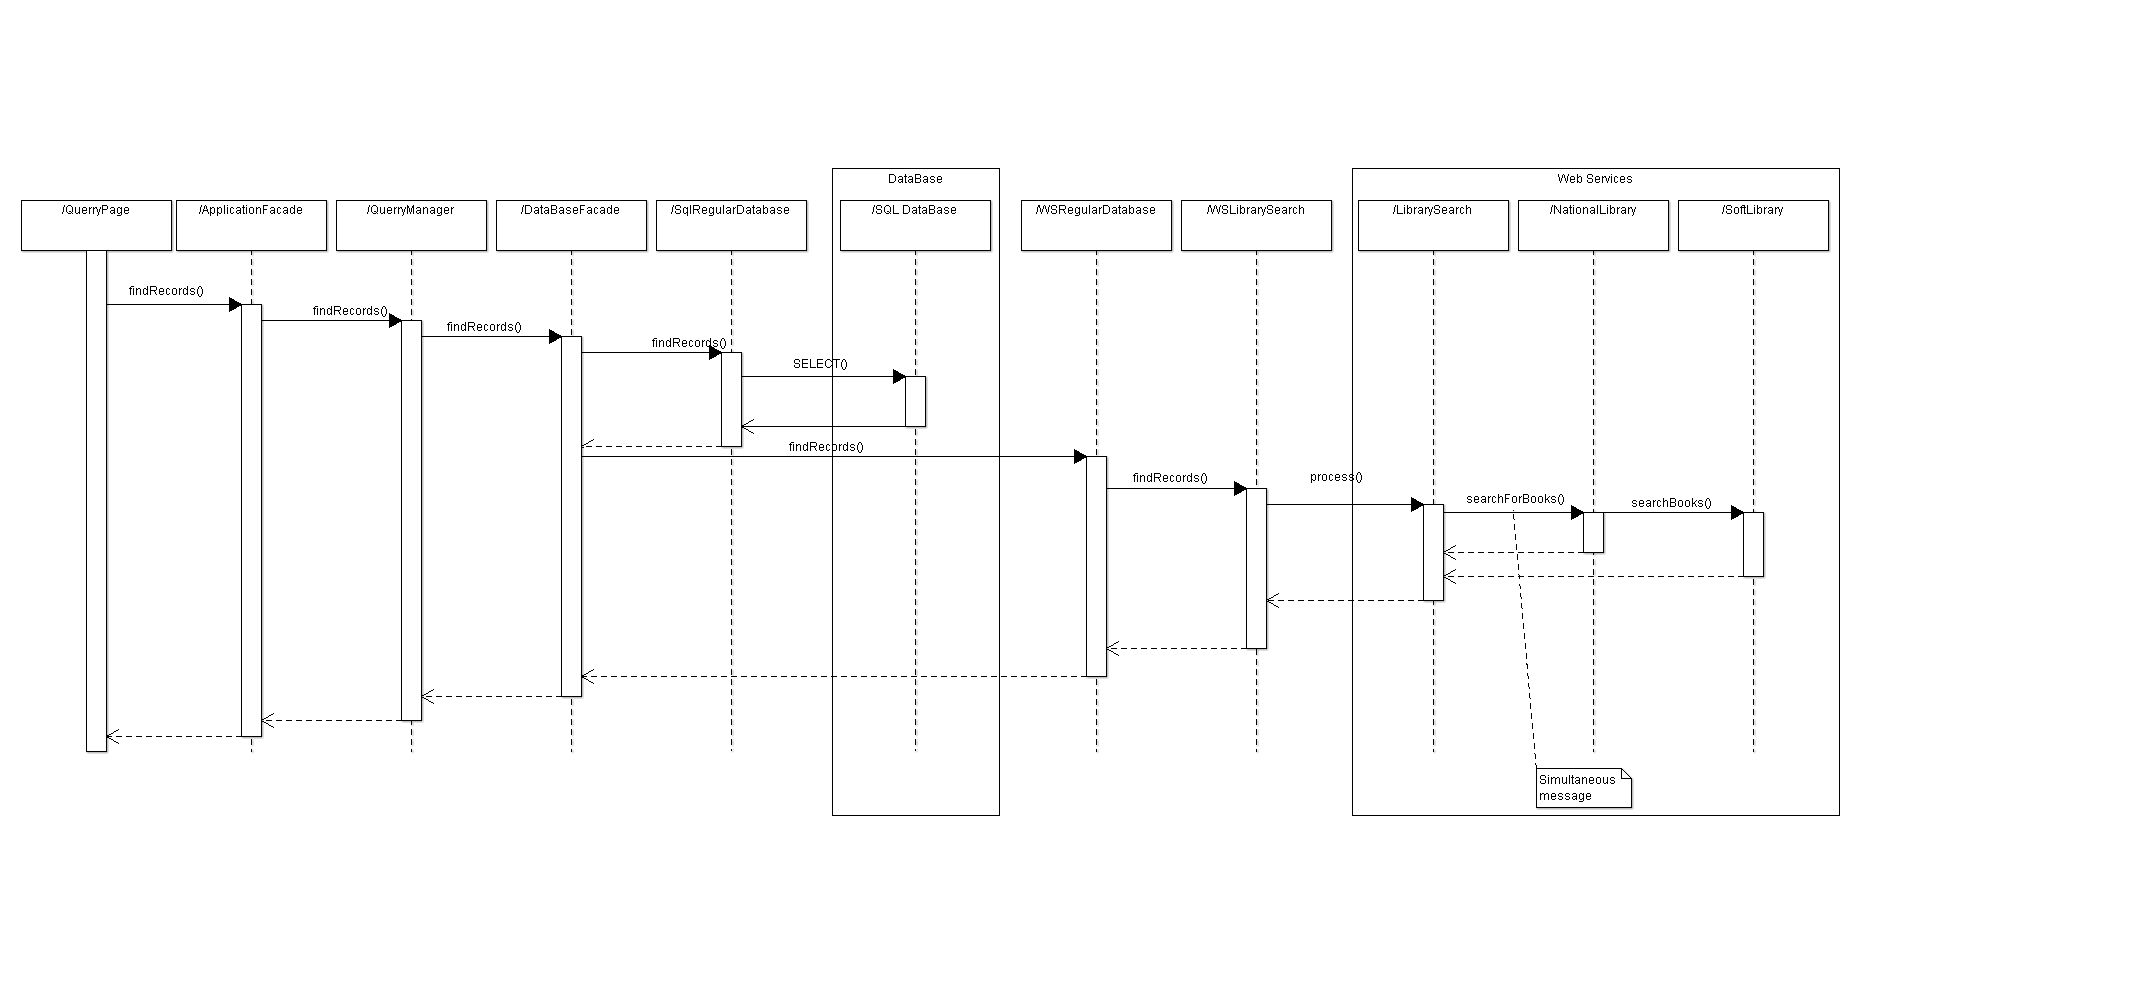
\includegraphics[scale=0.4]{uml/sequence.png}
   \caption{\label{sequence} Sequence diagram}
\end{figure}
\end{landscape}
This diagram is a sequence diagram which, in our case, allow us to see the exchange between the different part of the application. The diagram shows which part of the program are called when the user search for a book. We can notice that the function goes through different class due to some patterns, then arrive in the DataBaseFacade object in which two calls are performed, the first one is polling the local database (SQL in this case), the second one takes care of the web services. There is once again different class browsed until arrivin gin the WSLibrarySearch which querry the web service LibrarySearch using generated class. Finally, LibrarySearch invokes simultaneously the two library web services.
\end{document}
